% 04-mazequality.tex — maze_quality 八维几何度量

\section{maze\_quality 八维几何度量}
\label{sec:mazequality}

\subsection{设计原则}
\label{sec:mq-design}

记网格 $G \in \{0,1\}^{W\times H}$,其中 0 = 墙,1 = 通道,$|V| = N$ 为通道总数。
$maze\_quality$ 度量有以下四项设计原则 (源自源码
\texttt{src/metrics/maze\_quality.js} 文件头注释):

\begin{itemize}[leftmargin=*, itemsep=0pt, topsep=0pt]
  \item \textbf{无硬门 (no hard gate)}.
    所有子度量取值 $[0,1]$,连续可微,
    任意子度量的小幅提升都能反映到总分,
    ES 不会陷入 plateau。
  \item \textbf{抗单边 exploit}.
    经典 Bellot 2021 $F$ 度量对 ``单路径贯通'' 类反例给出高分;
    本度量采用两层加权几何聚合 + $\min$ 强制 balance,避免 ``高分
    topology + 低分 diversity'' 的 mode collapse。
  \item \textbf{拦截病态吸引子}.
    墙比软门控 $M_{\text{wall\_gate}}$ 在 $[0.40,\,0.60]$ 之外
    线性衰减,在 $[0,0]$ 与 $[1,1]$ 处为 0,
    避免 ``实心块'' (墙比 0) 与 ``空盒'' (墙比 1) 两种典型病态。
  \item \textbf{约定敏感}.
    度量按 ``1 = 通道 / 0 = 墙'' 计算,把同一图按 ``反'' 约定传入,所有
    拓扑子度量会崩塌为 0。这是双解读 (dual interpretation) 的根源
    (代码: \texttt{src/search/es\_searcher.js} 中 \texttt{withInvert}
    处理)。
\end{itemize}

\subsection{五个拓扑子度量}
\label{sec:5topo}

记 $V = \{v \in G : G(v) = 1\}$,$|V| = N$,并记 $v$ 的邻域度数为
$\deg(v) = \sum_{u \sim v} \mathbb{1}[G(u)>0]$。
公式直接对应源码
\texttt{src/metrics/maze\_quality.js::mBranching / mSpread / mJunction /
mConnectedness / mBoundary}。
\begin{align}
  M_b &= \mathrm{clip}\!\left(\frac{\#\{v \in V : \deg(v) = 2\}}{N} - 0.4,\, 0,\, 0.5\right) \big/ 0.5 \label{eq:mb}\\
  M_s &= \begin{cases}
    \dfrac{L_{\max}/N}{0.3}, & \text{if } L_{\max}/N \le 0.3 \\
    1 - \dfrac{L_{\max}/N - 0.5}{0.5}, & \text{if } 0.3 < L_{\max}/N \le 0.5 \\
    \max\!\left(0,\, 1 - \dfrac{L_{\max}/N - 0.5}{0.5}\right), & \text{if } L_{\max}/N > 0.5
  \end{cases} \label{eq:ms}\\
  M_j &= \exp\!\left[-\left(\dfrac{r_j - 0.10}{0.10}\right)^{2}\right], \quad r_j = \frac{\#\{v : \deg(v) \ge 3\}}{N} \label{eq:mj}\\
  M_c &= \frac{|C_{\max}|}{N} \big/ 0.8 \quad\text{(clipped to }[0,1]\text{)} \label{eq:mc}\\
  M_{\text{bnd}} &= \mathrm{clip}\!\left(1 - \dfrac{a_{\text{outer}} - 4}{76},\, 0,\, 1\right) \label{eq:mbnd}
\end{align}

其中 $L_{\max}$ 为图的 (4-邻) 最长路径长度,$C_{\max}$ 为最大 4-连通分量, 
$a_{\text{outer}}$ 为四条边上的活格子总数 (若 $a_{\text{outer}} \le 4$,$M_{\text{bnd}}=1$,
即 ``边界内层 4 个开口'' 的完美封闭评分)。

公式 (\ref{eq:mb}) 奖励 ``走廊主导'' (1-cell 宽直道):真 DFS 迷宫通常有 90\% 以上
的通道单元 $\deg=2$;\texttt{(ratio-0.4)/0.5} 把 0.5--0.9 区间线性映射到 [0,1],并截断
外侧。(\ref{eq:ms}) 在 $L_{\max}/N = 0.3$ 处达到峰值 1.0 并在 $[0.5, 1.0]$ 单调下降到 0,
故意惩罚 ``单路径贯穿'' 反例 (Spiral、Concentric Loop 等);这是抑制 Bellot $F$ 误判
的关键。(\ref{eq:mj}) 是以 $r_j=0.10$ 为峰的高斯钟形,因 ``走廊 + 适度分叉'' 是真迷宫
的特征:完全没有分叉是 Spiral,全是分叉是 noise blob。(\ref{eq:mc}) 把 ``最大连通分量
占比'' 截断到 0.8 即满分,允许最多 20\% 的 ``内部墙体孔洞'' 残留。(\ref{eq:mbnd}) 即
``外圈抑制'':典型真迷宫最多有 4 个边界开口 (入口与出口),其余必须是墙;典型 CA 退化解
``整张图外圈都是通道'' 会得 $M_{\text{bnd}}=0$,从而拖累 $M_{\text{topology}}$。

\subsection{三个多样性子度量}
\label{sec:3div}
\begin{align}
  M_p &= \frac{H(\text{2x2 patch})}{\log_2 16} \label{eq:mp}\\
  M_a &= \begin{cases}
    0.5, & \text{if } \max \mathrm{match}(G, G^{\text{flip}}) < 0.55 \\
    1.0, & \text{if } 0.55 \le \max \mathrm{match} < 0.85 \\
    \max\!\left(0,\, 1 - \dfrac{\max \mathrm{match} - 0.85}{0.15}\right), & \text{if } \max \mathrm{match} \ge 0.85
  \end{cases} \label{eq:ma}\\
  M_t &= \frac{H(\text{2x2 pair (cur, right)})}{\log_2 256} \label{eq:mt}
\end{align}

其中 $\mathrm{flip}$ 遍历 h-flip / v-flip / 180° 旋转;$\max \mathrm{match}(G, G^{\text{flip}})$
取三种对称下 ``活格子同位重合率'' 的最大值。
(\ref{eq:mp}) 采用 $2{\times}2$ 块的 Shannon 熵并除以 $\log_2 16=4$ 得到归一化值;真迷宫
通常达到 0.85--0.95,条纹类反例仅 0.2--0.4。
(\ref{eq:ma}) 双门控设计:
$\max \mathrm{match} \in [0.55, 0.85]$ 给出满分 1.0 (真迷宫的非对称形态),
$<0.55$ 取 0.5 (纯随机) 且被 $M_c$ 二次过滤,
$\ge 0.85$ 线性衰减 (周期性 / 高度对称会失分)。
(\ref{eq:mt}) 取 ``当前 $2{\times}2$ 块 + 右侧 $2{\times}2$ 块'' 的 256 维 Shannon 熵,
惩罚 ``小尺度低频重复'' (fractal tree、horizontal stripes)。

\subsection{二层聚合}
\label{sec:agg}

拓扑侧 (五维) 与多样性侧 (三维) 各自做加权几何聚合;两侧再取 $\min$ 强制 balance;最终
乘以墙比软门控。形式地:
\begin{align}
  M_{\text{topology}} &= M_b^{0.10} \cdot M_s^{0.10} \cdot M_j^{0.10} \cdot M_c^{0.40} \cdot M_{\text{bnd}}^{0.30} \label{eq:topo}\\
  M_{\text{diversity}} &= M_p^{0.25} \cdot M_a^{0.25} \cdot M_t^{0.50} \label{eq:div}\\
  M_{\text{wall\_gate}} &= \begin{cases}
    M_{\text{wall}} / 0.40, & M_{\text{wall}} \in [0, 0.40] \\
    1.0, & M_{\text{wall}} \in [0.40, 0.60] \\
    (1 - M_{\text{wall}}) / 0.40, & M_{\text{wall}} \in [0.60, 1.0] \\
    0, & M_{\text{wall}} \in \{0, 1\}
  \end{cases} \label{eq:gate}\\
  M_{\text{maze}} &= \min\!\left(M_{\text{topology}},\, M_{\text{diversity}}\right) \cdot M_{\text{wall\_gate}} \label{eq:final}
\end{align}

权重选择有明确的瓶颈识别动机。
(\ref{eq:topo}) 中 $M_c$ 取 0.40 (走廊结构的最强信号),$M_{\text{bnd}}$ 取 0.30 (外圈
抑制在 0.7591 引诱吸引子分析后新增),其余三个各 0.10;
(\ref{eq:div}) 中 $M_t$ 取 0.50,因经验上 $M_t$ 是多样性侧的最弱项,提高其权重使 ES
可见梯度。

$\min$ 而非几何均值,是与 Bellot $F$ 最关键的区别:
单边 exploit (高 $M_c$ 但低 $M_t$) 在几何均值下被宽松放过
($\sqrt{0.9 \cdot 0.1} \approx 0.30$),
而 $\min$ 强制 $M_{\text{base}} \le 0.1$,从而拖累总分。
此处 $M_{\text{base}}$ 不是 ``硬门'' ($M_{\text{base}}=0$ 在 $M_t>0$ 时不存在),
而是一种 ``结构性 balance'' (短板决定分数,
迫使 ES 同步提升两侧)。

$M_{\text{wall\_gate}}$ 的三角峰值 $[0.40,\,0.60]$ 与迷宫典型 ``道路占比 $40\%$
$\!\sim\!60\%$'' 的密度相符 (6 个真迷宫生成器的均值 $M_{\text{wall}}=0.487$ 落在
峰值中点)。把这一比例纳入聚合,等价于告诉 ES ``你要接近这个密度才有奖励''
而非 ``必须落在一条线上''。

\begin{figure}[H]
\centering
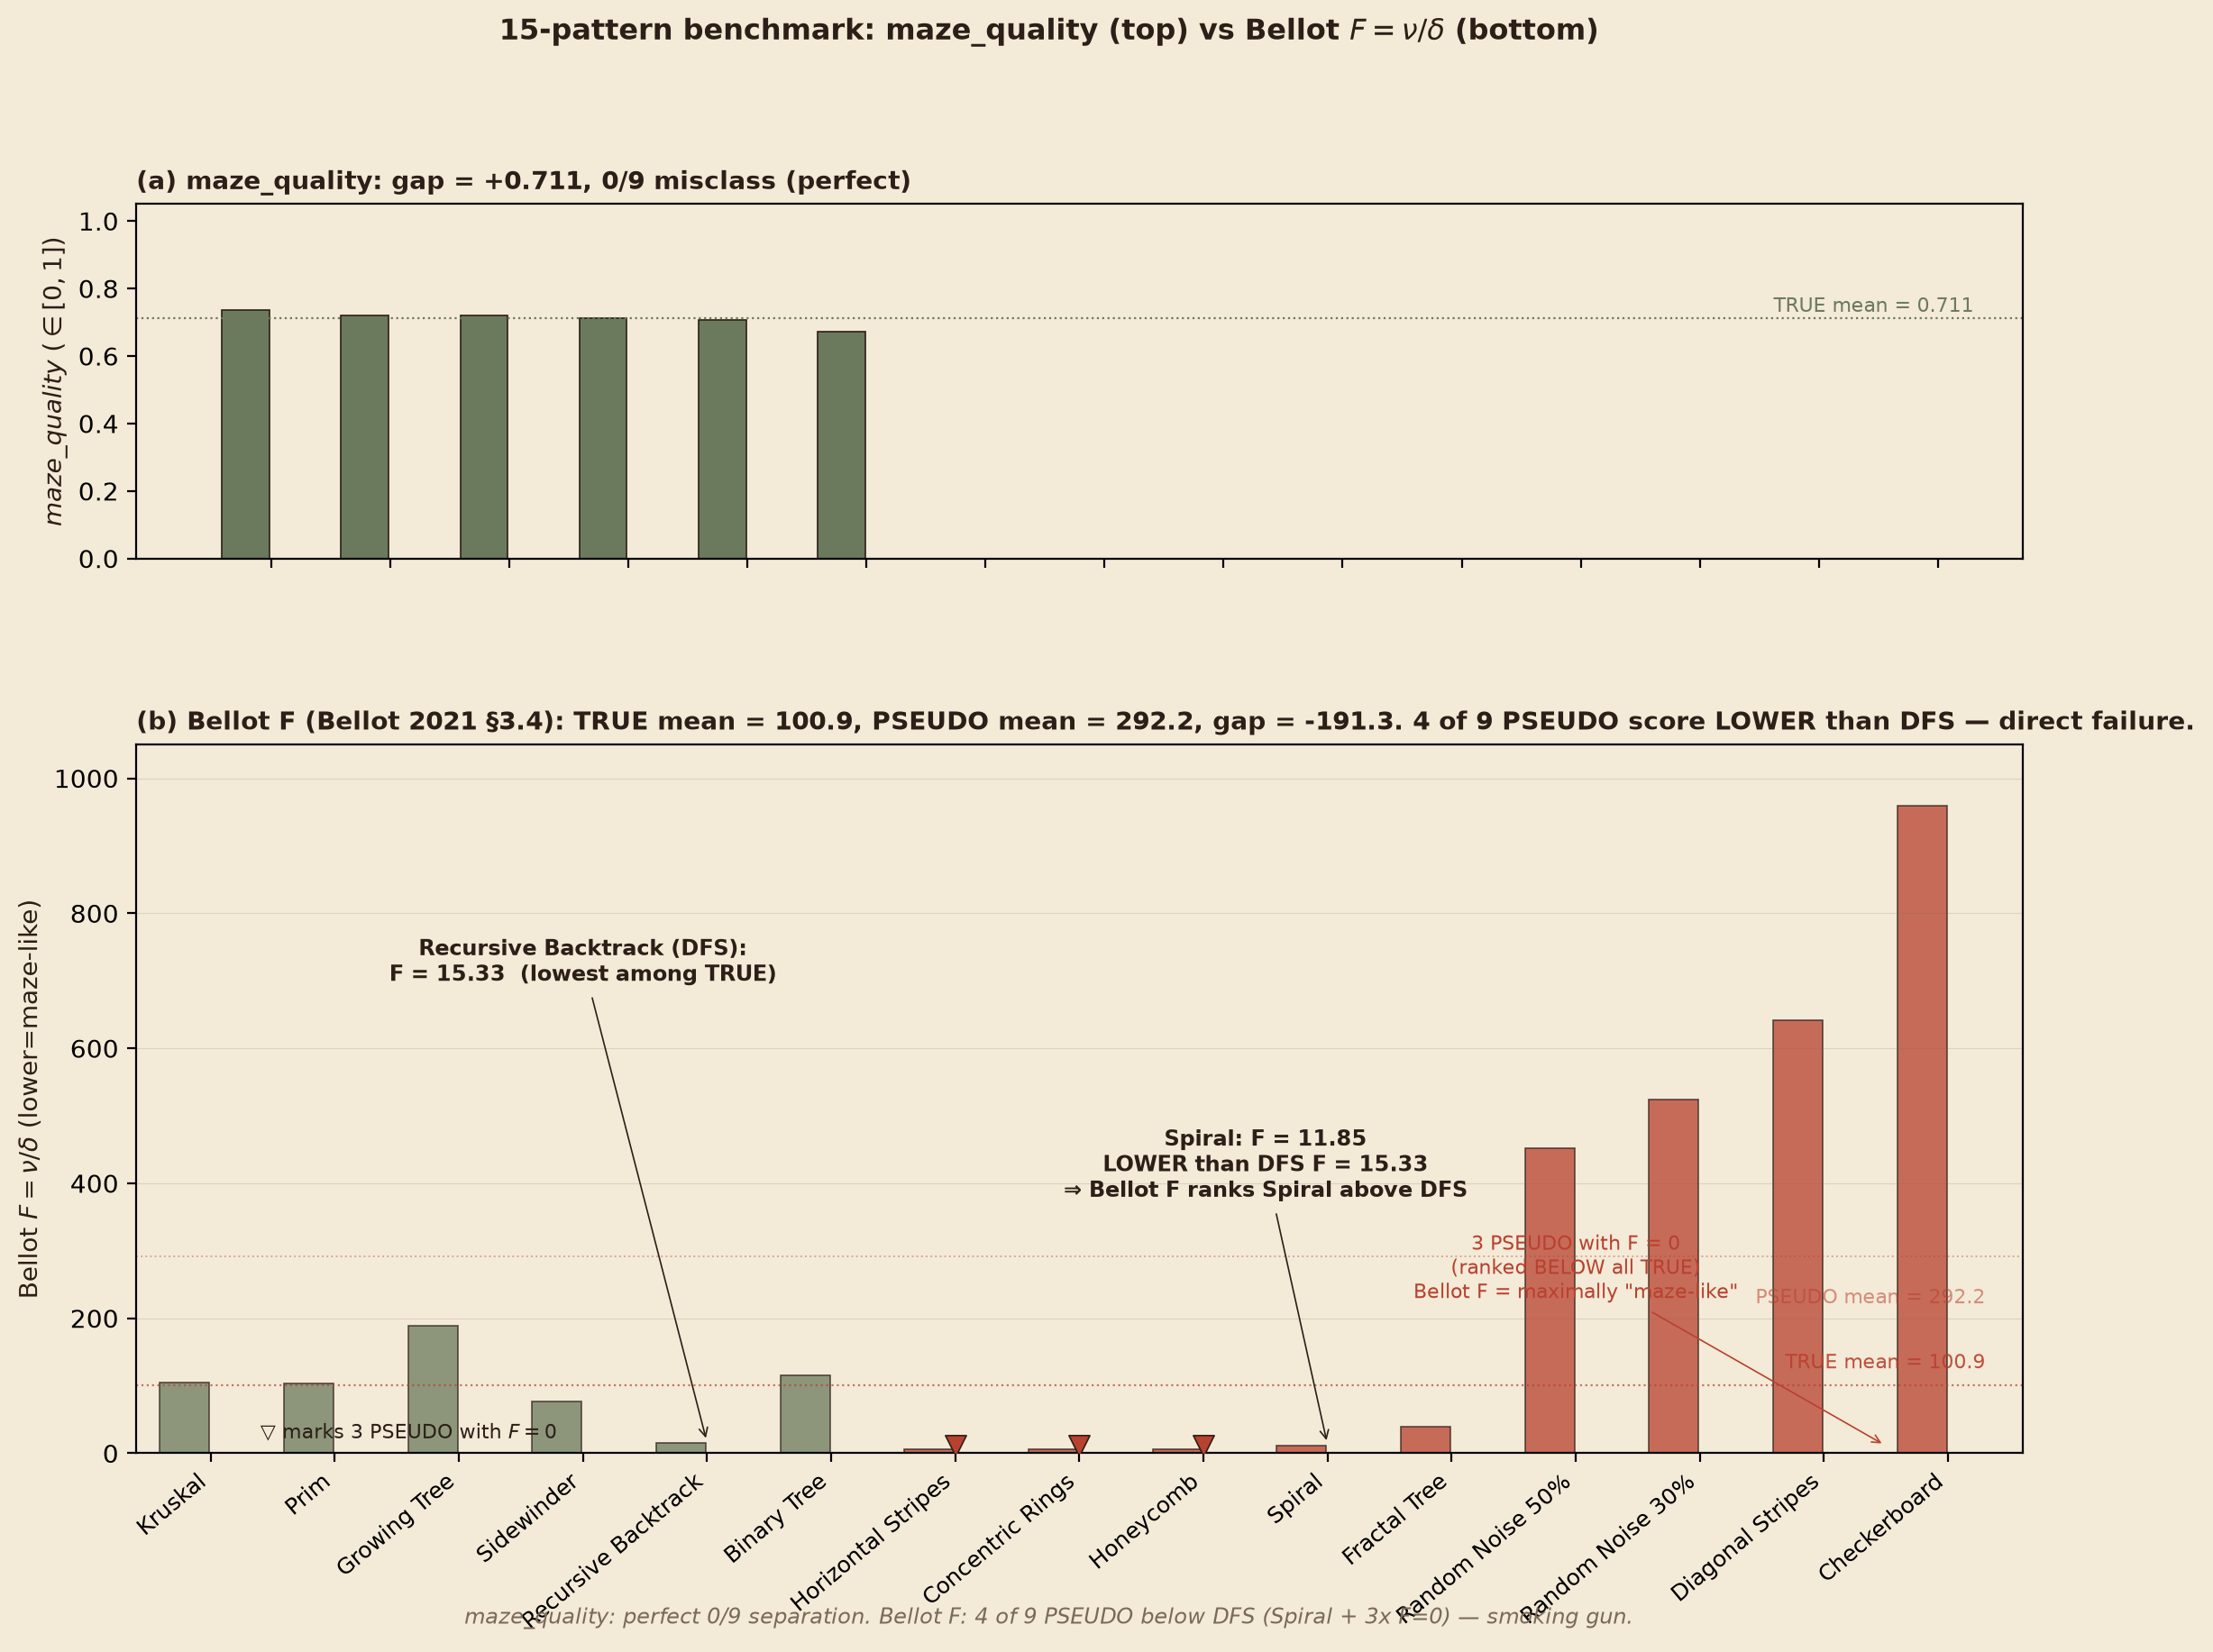
\includegraphics[width=0.96\linewidth]{figures/fig_15pattern.png}
\caption{\textbf{maze\_quality vs Bellot 2021 $F$ 在 15-pattern 数据集上的对比。}
深绿 (olive) 为 6 个真迷宫生成器;朱红为 9 个几何反例 (Spiral、Fractal Tree、
Horizontal Stripes、Random Noise (50\% / 30\%)、Checkerboard、Diagonal Stripes、
Concentric Rings、Honeycomb);前者均值 $0.711$,后者均值 $0.000$,间隔 $+0.711$,
9 个伪迷宫被全部拒收;Bellot $F = \nu/\delta$ 真伪间隔 $-191.3$,方向相反
(值越小越``像迷宫'',由 $\nu = $ 非显著墙计数,$\delta$ = twistiness proxy 决定)。
在 smoking gun 段,Spiral $F = 11.85$ 显著低于 Recursive Backtrack $F = 15.33$,
即 ``Spiral 比 DFS 更像迷宫'';另外 3 个伪迷宫 (Horizontal Stripes、
Concentric Rings、Honeycomb) $F = 0$,Bellot F 把它们判为``最像迷宫'' (比 DFS
还像)。整体 9 个伪迷宫中有 4 个排名反低于真迷宫最低值,误判率
非平凡 (\textit{smoking gun,见附录~D 系统审计 (\texttt{tab:repro-audit})})。
}
\label{fig:15pat}
\end{figure}
